\documentclass{llncs}

%\usepackage{makeidx}  % allows for indexgeneration
\usepackage{graphicx}

\begin{document}

\title{SWAML, from Mailing Lists to the Semantic Web}

\titlerunning{SWAML, from Mailing Lists to the Semantic Web}


\author{
Sergio Fern\'andez \and Diego Berrueta \and Jose E. Labra
}


\authorrunning{Sergio Fern\'andez et al.}

\tocauthor{Sergio Fern\'andez, Diego Berrueta, Jose E. Labra (Universidad de Oviedo)} 

\institute{Universidad de Oviedo, \\
Technical School of Computer Science, \\
Oviedo, Asturias, Spain,\\
\email{sergio@wikier.org, diego@berrueta.net, labra@uniovi.es},\\
WWW home page: \texttt{http://swaml.berlios.de/}
}

\date{1 February 2007}

\maketitle

\begin{abstract}

Mailing list archives (i.e., the messages posted up-to-now) are often published 
on the web and indexed by conventional search engines. They store a vast 
knowledge capital. However, the ability to auto-matically recognize and process 
the information is mostly lost at publishing time. As a result, the current 
mailing list archives are hard to query and have a limited use. This paper 
describes how SWAML uses Semantic Web technologies in order to avoid the
information loss and to allow new applications able to exploit this 
information in a more convenient way.

\end{abstract}

\section{Introduction}

FIXME

\subsection{SIOC}

SIOC (Semantically-Interlinked Online Communities) provides methods for 
interconnecting discussion methods such as blogs, forums and mailing lists 
to each other. It consists of the SIOC ontology, an open-standard machine 
readable format for expressing the information contained both explicitly 
and implicitly in internet discussion methods, of SIOC metadata producers 
for a number of popular blogging platforms and content management systems, 
and of storage and browsing/searching systems for leveraging this SIOC 
data. \cite{Breslin2005}

The goal of SIOC \footnote{\url{http://sioc-project.org/}} is to interconnect
these online communities. Community sites can include many discussion primitives,
such as bulletin boards, weblogs and mailing lists, which it have grouped under 
the concept of forum.

\begin{figure}[ht]
 \centering
 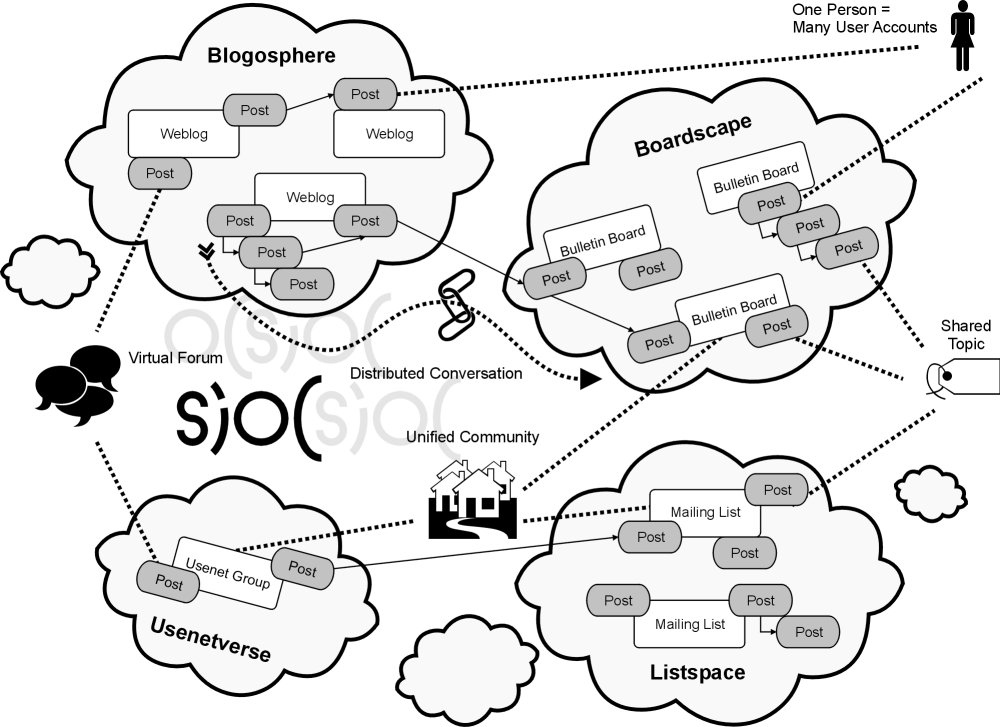
\includegraphics[bb=0 0 240 174]{images/sioc-discussion.png}
 \caption{Connections between discussion clouds with SIOC}
\end{figure}

FIXME: talk about SIOC classes?

FIXME: wrappers to existing tools (legacy systems y Web-based systems) 
in \cite{Breslin2005} (point 3.1).

\section{Components}

FIXME

\subsection{SWAML}

FIXME

\subsection{Buxon}

FIXME

\section{Conclussions and Future Work}

FIXME, interesting stuff here...


\bibliographystyle{abbrv}
\bibliography{../references}
%
\end{document}
